\documentclass{article}
\usepackage[margin=1in]{geometry}
\usepackage[shortlabels]{enumitem}
\usepackage{tikz}
\usetikzlibrary{automata, arrows}
\usetikzlibrary{shapes.multipart}

\begin{document}

\begin{center}
\bf\Large State Machine Proposal \\\smallskip
\rm\normalsize 25 Wednesday 2017
\rule{\textwidth}{1pt}
\end{center}

\section*{State Machine Overview}

The purpose of this state machine is to allow for robust high-level control of the Beluga robot, as well as a safe way to handle errors during operation. \\

\noindent The proposed states are as follows:
\vspace{3pt}
\begin{itemize}[nosep]
\item {\bf Initial:}
  This is the initial state of the robot when it is turned on.
  In this state, the robot waits for user input to determine what to do next, and does not run any motors.
  The robot can be put into this state from any other state with a reset command from the user.
\item {\bf Trajectory Tracking:}
  This is the state for standard operation.
  The robot will track the given trajectory until it reaches the end of the path, and then the robot will transition to the park state.
  If the robot encounters an error during trajectory tracking, the robot will transition to the idle recovery state.
\item {\bf Park:}
  In this state, the robot will attempt to stay in place (within a small radius) while sitting on the surface of the water.
  If the robot's position estimate becomes too uncertain (i.e. covariance is too high) or we encounter another error, the robot will transition to the idle recovery state.
\item {\bf Drive-By-Wire:}
  This is the user-controlled drive state.
  In this state, the user is able to control the robot on the surface with a joystick (or arrow keys).
  If we lose connection with the robot, we will transition into the idle recovery state.
\item {\bf Idle Recovery:}
  This is the general purpose recovery state.
  In this state, the robot will float to the surface and then determine if it is possible to park the robot.
  If we are on the surface with a small position covariance and we have enough battery, the robot will transition into the park state.
  During this process, the robot will be broadcasting the errors that forced it into this state (see the error handling section).
\end{itemize}

\begin{figure}[h]
\centering
\resizebox{0.6\linewidth}{!}{
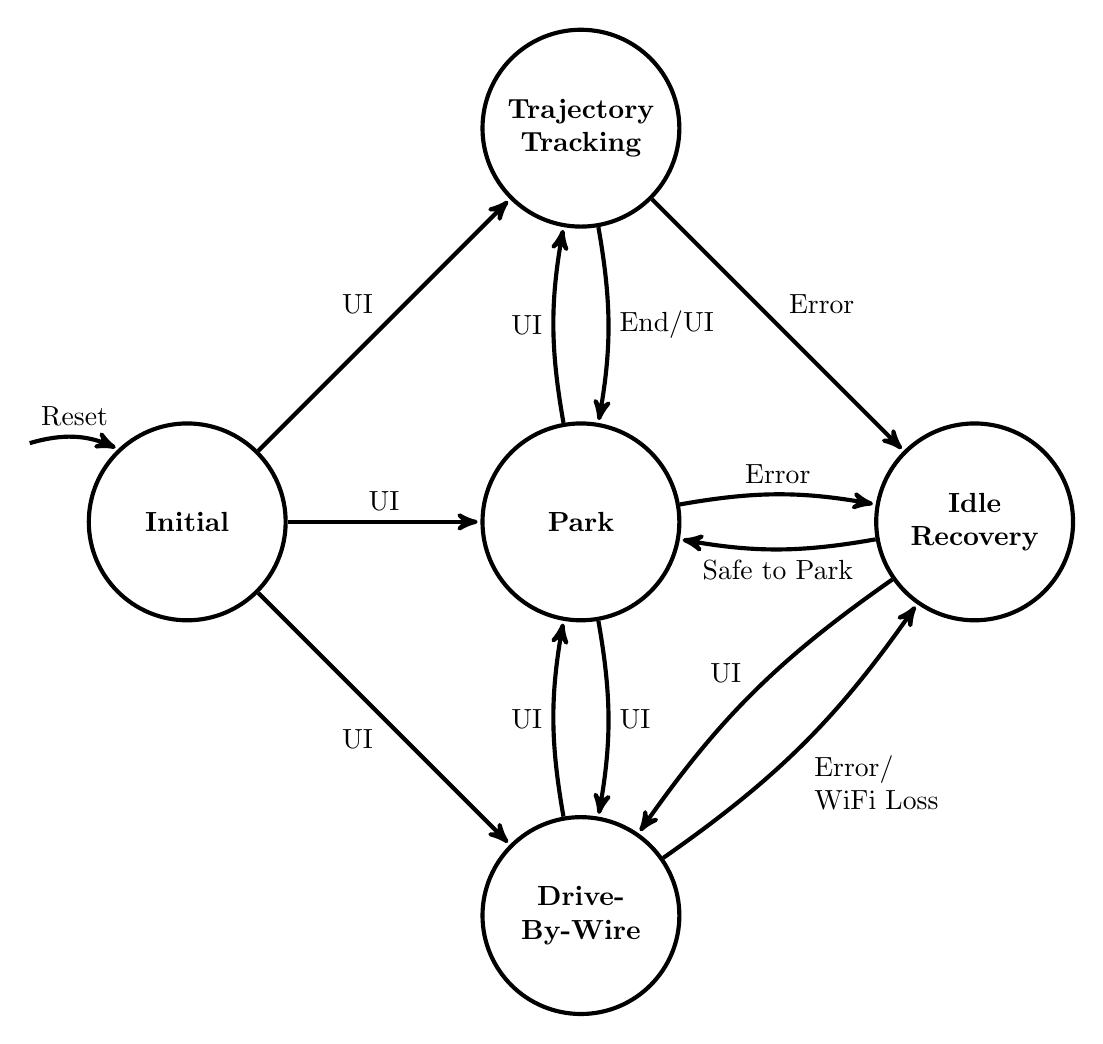
\begin{tikzpicture}[x=1cm,y=1cm,>=stealth',shorten >=1pt,auto,line width=1.5pt]
\tikzset{state/.style = {shape=circle, draw, minimum size=2.5cm,line width=1.5pt}}

%states
\node[state] (init) at (0,0) {\bf Initial};
\node[state] (traj) at (5,5) [text width=2cm,align=center] {\bf Trajectory Tracking};
\node[state] (park) at (5,0) [text width=2cm,align=center] {\bf Park};
\node[state] (drive) at (5,-5) [text width=2cm,align=center] {\bf Drive-By-Wire};
\node[state] (idle) at (10,0) [text width=2cm,align=center] {\bf Idle Recovery};
\coordinate (reset) at (-2,1);

%transitions
\path[->] (reset) edge [bend left=20] node[above] {Reset} (init);

\path[->] (init) edge  node {UI} (traj);
\path[->] (init) edge node [swap] {UI} (drive);
\path[->] (init) edge node {UI} (park);

\path[->] (drive) edge [bend left=10] node {UI} (park);
\path[->] (drive) edge [bend right=10] node [swap,text width=2cm] {Error/\\ WiFi Loss} (idle);

\path[->] (park) edge [bend left=10] node {UI} (drive);
\path[->] (park) edge [bend left=10] node {Error} (idle);
\path[->] (park) edge [bend left=10] node {UI} (traj);

\path[->] (traj) edge [bend left=10] node {End/UI} (park);
\path[->] (traj) edge node {Error} (idle);

\path[->] (idle) edge [bend left=10] node {Safe to Park} (park);
\path[->] (idle) edge [bend right=10] node [swap] {UI} (drive);

\end{tikzpicture}
}
\caption{The proposed state machine for high level control of the Beluga}
\end{figure}

\section*{Possible Additional States}
The team also discussed possible additional states that could be implemented, but weren't included in this draft of the state machine:
\vspace{3pt}
\begin{itemize}[nosep]
\item {\bf Surface:}
This would be an active surfacing state, where the Beluga uses its motors to bring itself up to the surface.
In the current state machine, the robot will just float to the surface (assuming it is slightly positively buoyant).
\item {\bf Safe Return Path:}
This would be an alternative to the idle recovery state where the robot would drive itself back to a known location along a know safe path (given to the robot along with its desired trajectory).
In the current state machine, the robot will attempt to park itself in place on the surface if it receives an error.
\end{itemize}

\section*{Error Handling}
Along with the proposed state machine, we are also proposing a separate error handling system.
This system will receive error messages from other nodes and keep a queue of errors.
The system will then repeatedly publish all errors in the queue until the user's machine acknowledges that it has received the messages.
This allows the state machine to queue error messages and then change states without needing to worry about whether or not the user has received those error messages. \\

\noindent The proposed initial list of possible errors is as follows:
\vspace{3pt}
\begin{itemize}[nosep]
\item {\bf Low Battery:} We will be monitoring the battery levels, and if it goes too low we will raise this error. We will also raise this error if we don't have enough battery to make it the point we're trying to get to.
\item {\bf Sensor Errors:} If we lose connection with a sensor or stop receiving data, we will raise one of these errors. If we need that sensor for operation in the current state, we will also trigger a state transition.
\item {\bf Stuck:} If the robot is not moving in the direction that we expect it to over the span of a few (maybe 5) seconds, we will assume it is stuck, raise this error, and stop moving.
\item {\bf Waypoint too far away:} In trajectory tracking, if the point we are trying to send the robot to is too far away (i.e. trying to send the robot at Catalina to the Scripps pool), we will raise this error and abort.
\item {\bf Moisture:} If we detect moisture inside the robot, we raise this error (and surface if necessary).
\item {\bf WiFi loss:} If we lose WiFi connection during communication with the robot when we don't expect to, we raise this error (most likely only in drive-by-wire and initial)
\end{itemize}

\section*{State Machine Implementation}
The state machine would be implemented as as single publisher/subscriber node.
It would contain all of the state transition logic and constantly publish the current state.
It would also subscribe to all of the nodes that can trigger state transitions.

\end{document}
